\section{Results}\label{sec:results}

We first examined whether greater surface flexibility and narrower parameter sharing improved the fit to observed IV. The filtered corpus contained 234{,}549 observations from 31 tickers across fifteen snapshots and six market groups (Supplementary Tables~\ref{tab:sector_map} and~\ref{tab:corpus_dates}). We fitted global parametric, global neural, and sector-specific neural shapes using the same loss and retaining ticker-specific levels in every model. Root mean squared error (RMSE) measured agreement with reported IV in volatility percentage points, with lower values indicating a closer fit. Replacing the global parametric shape with a global neural surface reduced pooled in-sample error from 12.48 to 11.47 points, and sector-specific networks reduced it further to 10.24 points (Table~\ref{tab:three_way}). The sector gains extended across all six groups and were largest in exchange-traded funds (ETFs) and financials (Supplementary Table~\ref{tab:per_sector}). Technology and healthcare nevertheless retained the largest errors and contained the weakest individual ticker fits (Supplementary Table~\ref{tab:worst_tickers}). These remaining differences motivated separate surfaces for tickers with sufficient observations. Assigning per-ticker networks where the sample threshold was met reduced pooled error to 9.73 points while retaining sector fits for the remaining tickers (Table~\ref{tab:three_way}). Most qualified tickers improved under this change (Supplementary Table~\ref{tab:per_ticker_comparison}). The smile panels nevertheless showed that lower pooled error did not ensure agreement on an individual date (Fig.~\ref{fig:per_ticker_panels}). Their observations came from May 11, while all three displayed surfaces had been fitted across fifteen snapshots. Near the money, the per-ticker fits exceeded observed IV by an average of 9.45 percentage points for MSFT and 7.90 points for LLY. The corresponding biases were small for SPY and GS, while AVGO was underpredicted by 5.37 points (Supplementary Table~\ref{tab:smile_date_bias}). These discrepancies were present in predictions at the observed contracts. A surface with moneyness and maturity as its only inputs could not adjust its level independently for May 11. Thus, greater flexibility and narrower sharing improved the pooled fit but left substantial date-specific errors. The interpretation rested on predicted IV because the ticker level and neural output bias were not separately identified in~\eqref{eq:sigma_model}. Lower error on the calibration observations alone did not establish more accurate option prices or better performance on future dates.

\begin{table}[H]
\centering
\caption{In-sample IV RMSE on 234{,}549 observations, reported in volatility percentage points. Each model fitted one ticker level jointly with its shape parameters. The final row used per-ticker neural surfaces for the 29 qualified tickers and sector surfaces for PFE and BMY.}\label{tab:three_way}
\begin{tabular}{lrr}
\toprule
Model & RMSE & Reduction from parametric \\
\midrule
Parametric shape, global               & 12.48 & reference \\
Neural shape, global                   & 11.47 & 8.1\% \\
Neural shape, six sectors              & 10.24 & 17.9\% \\
Neural shape, per-ticker with fallback &  9.73 & 22.0\% \\
\bottomrule
\end{tabular}
\end{table}

\begin{figure}[H]
\centering

\includegraphics[width=\textwidth]{sections/figures/ladder_per_ticker_nn_smile_panels.pdf}
\caption{In-sample comparison of the implied volatility (IV) observed on May 11, 2026 with surfaces fitted across all fifteen calibration snapshots. Panels show (a) SPY, (b) NVDA, (c) MSFT, (d) LLY, (e) GS, and (f) AVGO, with 7, 7, 9, 11, 11, and 9 calendar days to expiry, respectively. Circles and diamonds distinguish reported call and put IV; solid, dashed, and dotted curves show per-ticker neural, sector neural, and global parametric fits. The legend applies to all panels. The MSFT and LLY fits overpredict IV near the money; Supplementary Table~\ref{tab:smile_date_bias} reports the corresponding errors.}\label{fig:per_ticker_panels}
\end{figure}

To examine the pricing consequences of the fitted surfaces, we passed their IV predictions to the American lattice and compared the resulting values with observed option mids. The May 11 capture provided contracts for which dollar errors could also be judged against the local bid--ask half-spread. This comparison was needed because the same IV error can have different pricing consequences across contracts, and an improvement in pooled IV fit need not place a model price within the quoted spread. Only about one third of fitted SPY, NVDA, and LLY prices fell within the half-spread around the mid, compared with 88\% for GS (Fig.~\ref{fig:price_error}; Supplementary Table~\ref{tab:price_error_summary}). The largest median absolute error occurred in LLY at \$4.01 per share. To distinguish the contribution of the fitted IV input from the rest of the pricing calculation, we repeated the calculation with each contract's reported market IV in the same lattice. This substitution reduced the LLY median error to \$0.67 per share and pointed to a substantial contribution from the surface's date-specific IV level. The remaining errors also showed that the reported IV did not reproduce every captured mid under the American pricer. Since May 11 entered the full-corpus fits, these results described the pricing consequences of calibration error on an observed date. They established a reason to assess dollar-price accuracy alongside IV fit when evaluating the surface representation.

\begin{figure}[H]
\centering

\includegraphics[width=\textwidth]{sections/figures/ladder_price_error_three_tickers.pdf}
\caption{In-sample comparison of CRR American-option prices with market mids across moneyness for SPY, NVDA, LLY, and GS on May 11, 2026. Errors are lattice price minus market mid. Curves show the parametric, sector, per-ticker, and market-IV reference inputs. The gray ribbon is the median local bid--ask half-spread by moneyness bin. A point inside the ribbon has an absolute pricing error below that local half-spread.}\label{fig:price_error}
\end{figure}

We next examined whether the fitted surfaces transferred to withheld dates and whether earnings-calendar information improved that transfer. Removing May 11 and retraining the sector models on the other fourteen dates gave pooled error of 10.21 volatility percentage points on the training observations and 10.89 points on the holdout (Supplementary Table~\ref{tab:loo_sector_nn}). Energy and retail had the largest increases in error, so the modest pooled gap concealed differences among sectors. A separate temporal split then tested whether calendar inputs supplied information beyond moneyness and maturity. Configuration A used those two inputs alone, while Configuration C added distances to ticker and peer earnings dates on exactly the same training and test rows. The added inputs reduced error on the two-day holdout from 13.03 to 11.98 volatility percentage points (Table~\ref{tab:earnings_holdout}). Several technology tickers with nearby peer reports improved, although the gains did not extend to every ticker (Supplementary Table~\ref{tab:tech_pivot}). This comparison supported the usefulness of calendar information within the tested split. Configuration B examined the effect of removing observations near earnings before fitting the two-input model. Its similar training and test errors applied to the retained subset after most observations had been discarded. Because that filtering changed the composition of both samples, it could not attribute the original error gap to earnings alone. Every test ticker appeared in training, and neither temporal experiment covered repeated dates and training seeds. The results therefore supported limited transfer within the available window and a benefit from earnings inputs on one fixed holdout. They did not establish that the surfaces would retain the same accuracy across other market periods.

\begin{table}[H]
\centering
\caption{Temporal-holdout comparison. Training used six snapshots labeled April 14 through April 22, 2026, and testing used April 23--24; every test ticker appeared in training. Errors and gaps are in volatility percentage points. Configuration B used different row sets from A and C.}\label{tab:earnings_holdout}
\resizebox{\textwidth}{!}{%
\begin{tabular}{lrrrrr}
\toprule
Configuration & $N_{\mathrm{tr}}$ & $N_{\mathrm{te}}$ & Train RMSE & Test RMSE & Gap \\
\midrule
A: pooled, two inputs          & 103{,}897 & 26{,}833 & 8.05 & 13.03 & $+4.99$ \\
B: non-earnings, two inputs    &  29{,}383 &  4{,}516 & 8.02 &  7.96 & $-0.06$ \\
C: earnings-aware, four inputs & 103{,}897 & 26{,}833 & 7.61 & 11.98 & $+4.36$ \\
\bottomrule
\end{tabular}}
\end{table}

\FloatBarrier
Having evaluated the fitted surfaces, we used them to generate complete contract paths and examine how the stock and IV inputs entered American-option valuation. We selected one put and one call for each of GS and LLY from the April 28 capture with expiration on May 29 (Supplementary Tables~\ref{tab:gs_scenario} and~\ref{tab:lly_scenario}). The initial illustrations used 1{,}000 stock paths per ticker and a separate IV factor for each contract under the fixed settings in Supplementary Table~\ref{tab:scenario_settings}. Each factor followed a moving target supplied by the fitted surface before its IV entered the lattice calculation at the current stock price and remaining maturity. The GS paths showed the expected inverse relation between terminal stock and put payoff and the direct relation between terminal stock and call payoff (Fig.~\ref{fig:gs_paths}). Before expiration, the put and call factors followed different targets as moneyness and calendar days to expiration changed (Fig.~\ref{fig:gs_iv}). Their shared negative return coupling tended to increase factor shocks after lower standardized returns. The corresponding LLY paths demonstrated the same calculation under a different return marginal and higher fitted IV level (Supplementary Figs.~\ref{fig:lly_paths} and~\ref{fig:lly_iv}). The pathwise Greeks described the associated risk sensitivities through delta approaching the exercise states, gamma concentrating near the strike, and Vega declining toward expiration (Supplementary Figs.~\ref{fig:gs_greeks} and~\ref{fig:lly_greeks}). Algorithm~\ref{alg:forward_sim} describes these illustrations with return shocks standardized across the completed ensemble. The paired ablation used independent pilot constants instead, as described in Section~\ref{sec:ablation_methods}, to measure the contribution of IV dynamics on shared evaluation paths. Both experiments used surfaces fitted with observations from the scenario period and examined the behavior of the assembled model. They were illustrative scenarios, not forecasts evaluated against later observations; the chronological tests used separate fits and origins.

\begin{algorithm}[H]
\caption{Forward simulation of contract values}\label{alg:forward_sim}
\begin{algorithmic}[1]
\Require JumpHMM marginal; fitted $(\theta_i,\psi_i)$; contract $(K,T)$; trading dates $d_0,\ldots,d_L$; calendar DTE $\tau_0,\ldots,\tau_L$; $(\kappa,\sigma_v,\rho)$; $S_0$; $r$; $N_p$ paths; LR depth $N_{\mathrm{LR}}$.
\Ensure Stock, variance, IV, and option-value paths.
\State Draw $N_p$ JumpHMM stock paths with $L$ trading transitions.
\State Compute $Z^S_{j,\ell}$ by standardizing all simulated one-session log returns as in~\eqref{eq:return_shock}.
\State Draw $Z^\perp_{j,\ell}\sim\mathcal N(0,1)$ once per path and transition; set $Z^v_{j,\ell}\gets\rho Z^S_{j,\ell}+\sqrt{1-\rho^2}Z^\perp_{j,\ell}$ and reuse it for every contract.
\For{contract $a$ and path $j$}
  \State $v_{a,0}^{(j)} \gets \theta_i\psi_i(\tau_0,K/S_0)$
  \For{$\ell=0$ \textbf{to} $L-1$}
    \State $\sigma_{a,\ell}^{(j)} \gets \sqrt{v_{a,\ell}^{(j)}}$
    \State $P_{a,\ell}^{(j)} \gets \mathrm{LR}_{N_{\mathrm{LR}}}(S_{j,\ell},K,\sigma_{a,\ell}^{(j)},\tau_\ell/365,r)$
    \State $\bar v_{a,\ell}^{(j)}\gets\theta_i\psi_i(\tau_\ell,K/S_{j,\ell})$
    \State Update $v_{a,\ell+1}^{(j)}$ with the hard-floor rule in~\eqref{eq:euler} using $\Delta t=1/252$.
  \EndFor
  \State $P_{a,L}^{(j)}\gets\max\{\phi(S_{j,L}-K),0\}$, where $\phi=1$ for a call and $\phi=-1$ for a put.
\EndFor
\State \Return all paths.
\end{algorithmic}
\end{algorithm}

\begin{figure}[!htbp]
\centering
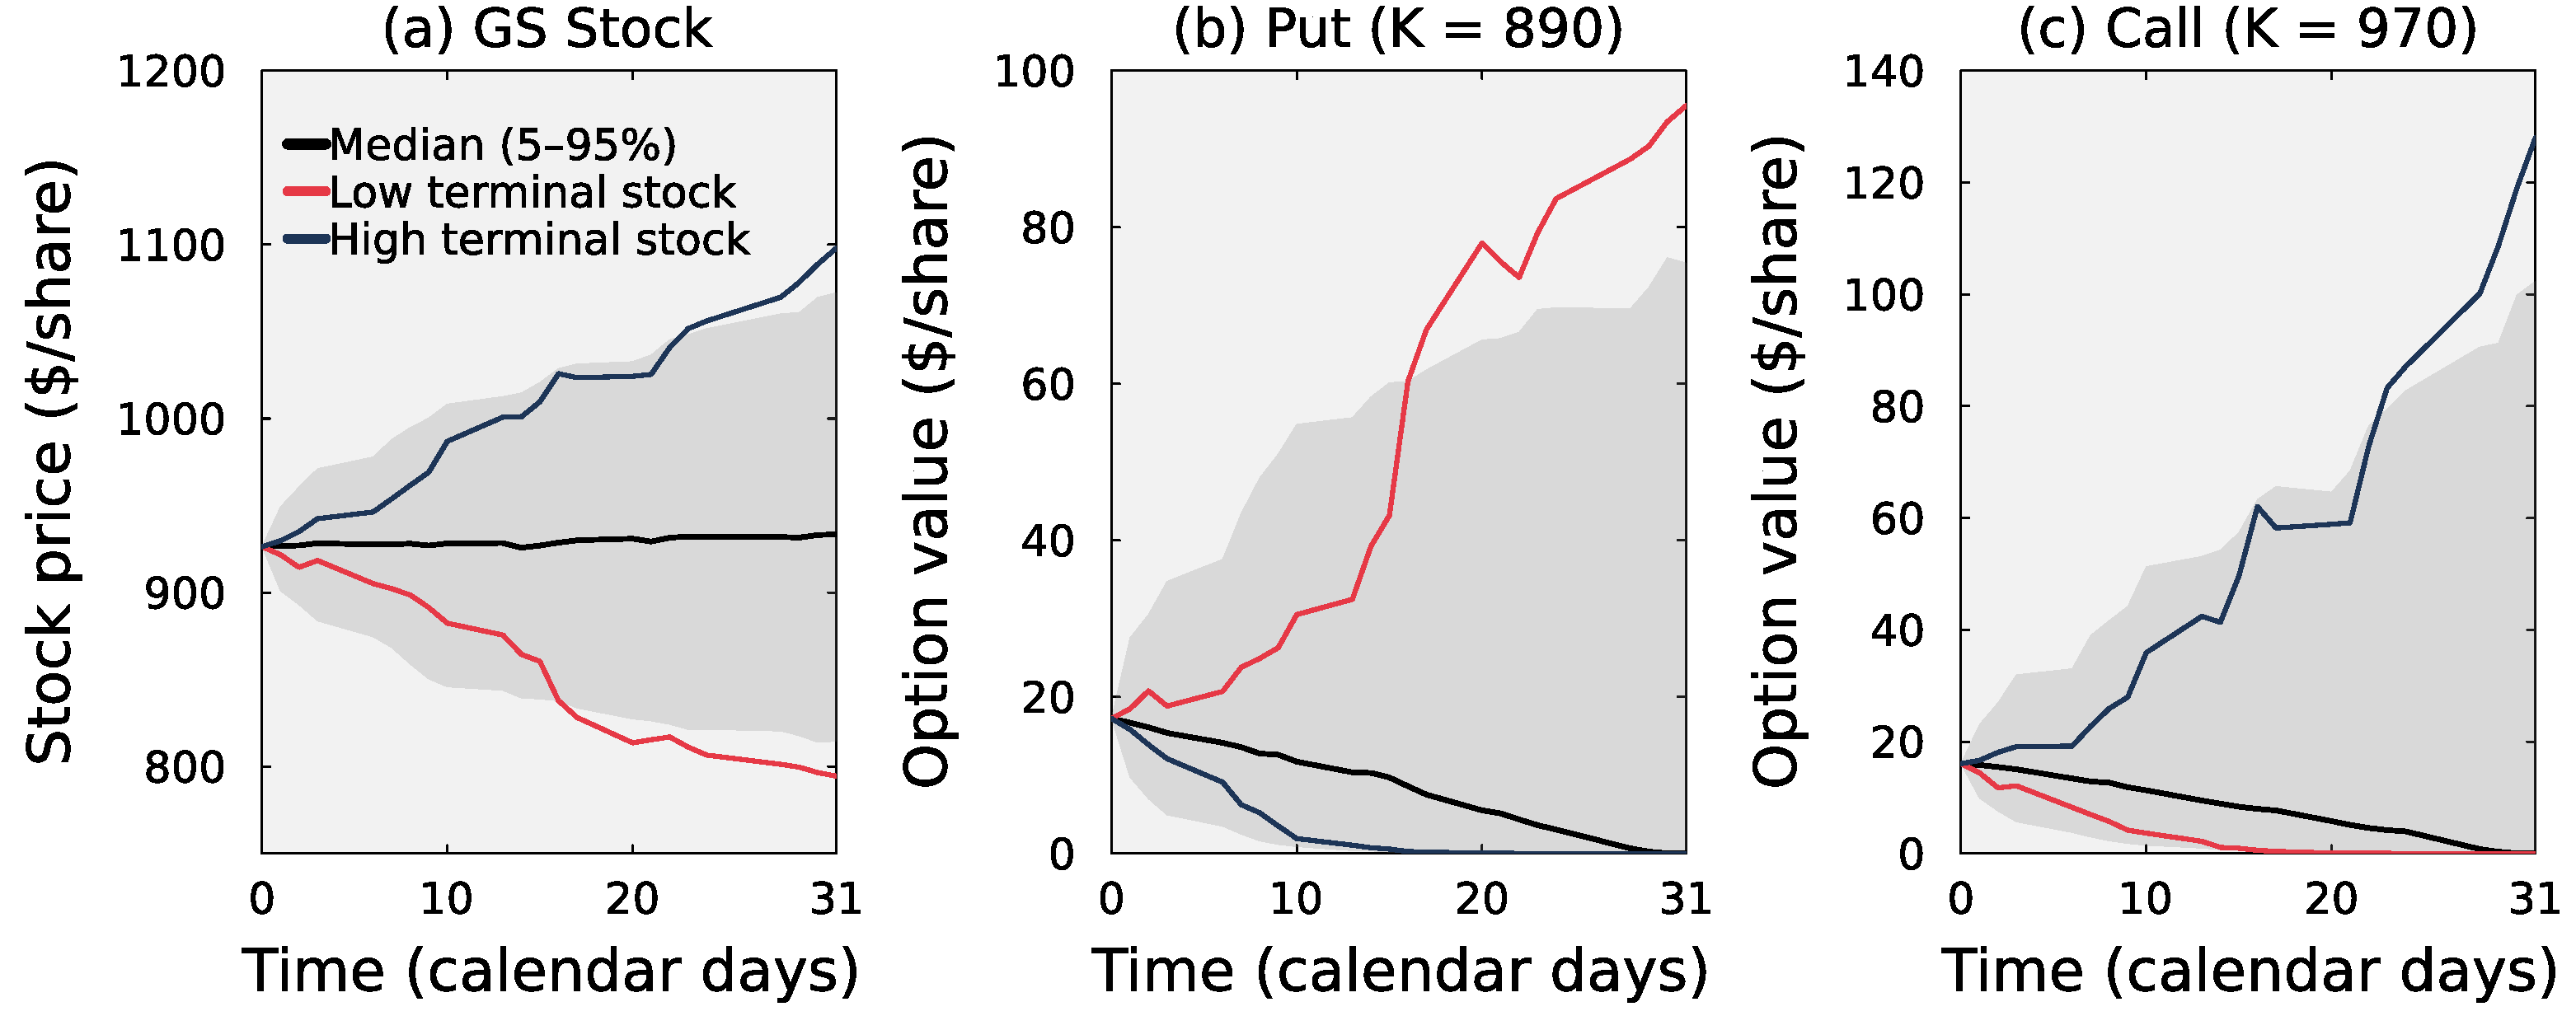
\includegraphics[width=\textwidth]{sections/figures/gs/gs_short_paths.pdf}
\caption{Simulated evolution of GS stock prices (a), put values (b), and call values (c) along 1{,}000 paths between April 28 and May 29, 2026. The fitted surfaces included observations from this scenario period, so these paths illustrate the model rather than an out-of-sample forecast. Time is measured in calendar days from April 28. Black curves show the median at each date, and shaded bands contain the middle 90\% of values. Red and blue curves show group medians for paths ranked in the 1st--5th and 95th--99th percentiles of terminal stock price. These summaries are not individual trajectories. Option values are dollars per share and represent the cost of repurchasing the contract for a short seller. Entry premiums were \$16.51 per share for the put and \$16.09 for the call.}
\label{fig:gs_paths}
\end{figure}

\begin{figure}[!htbp]
\centering
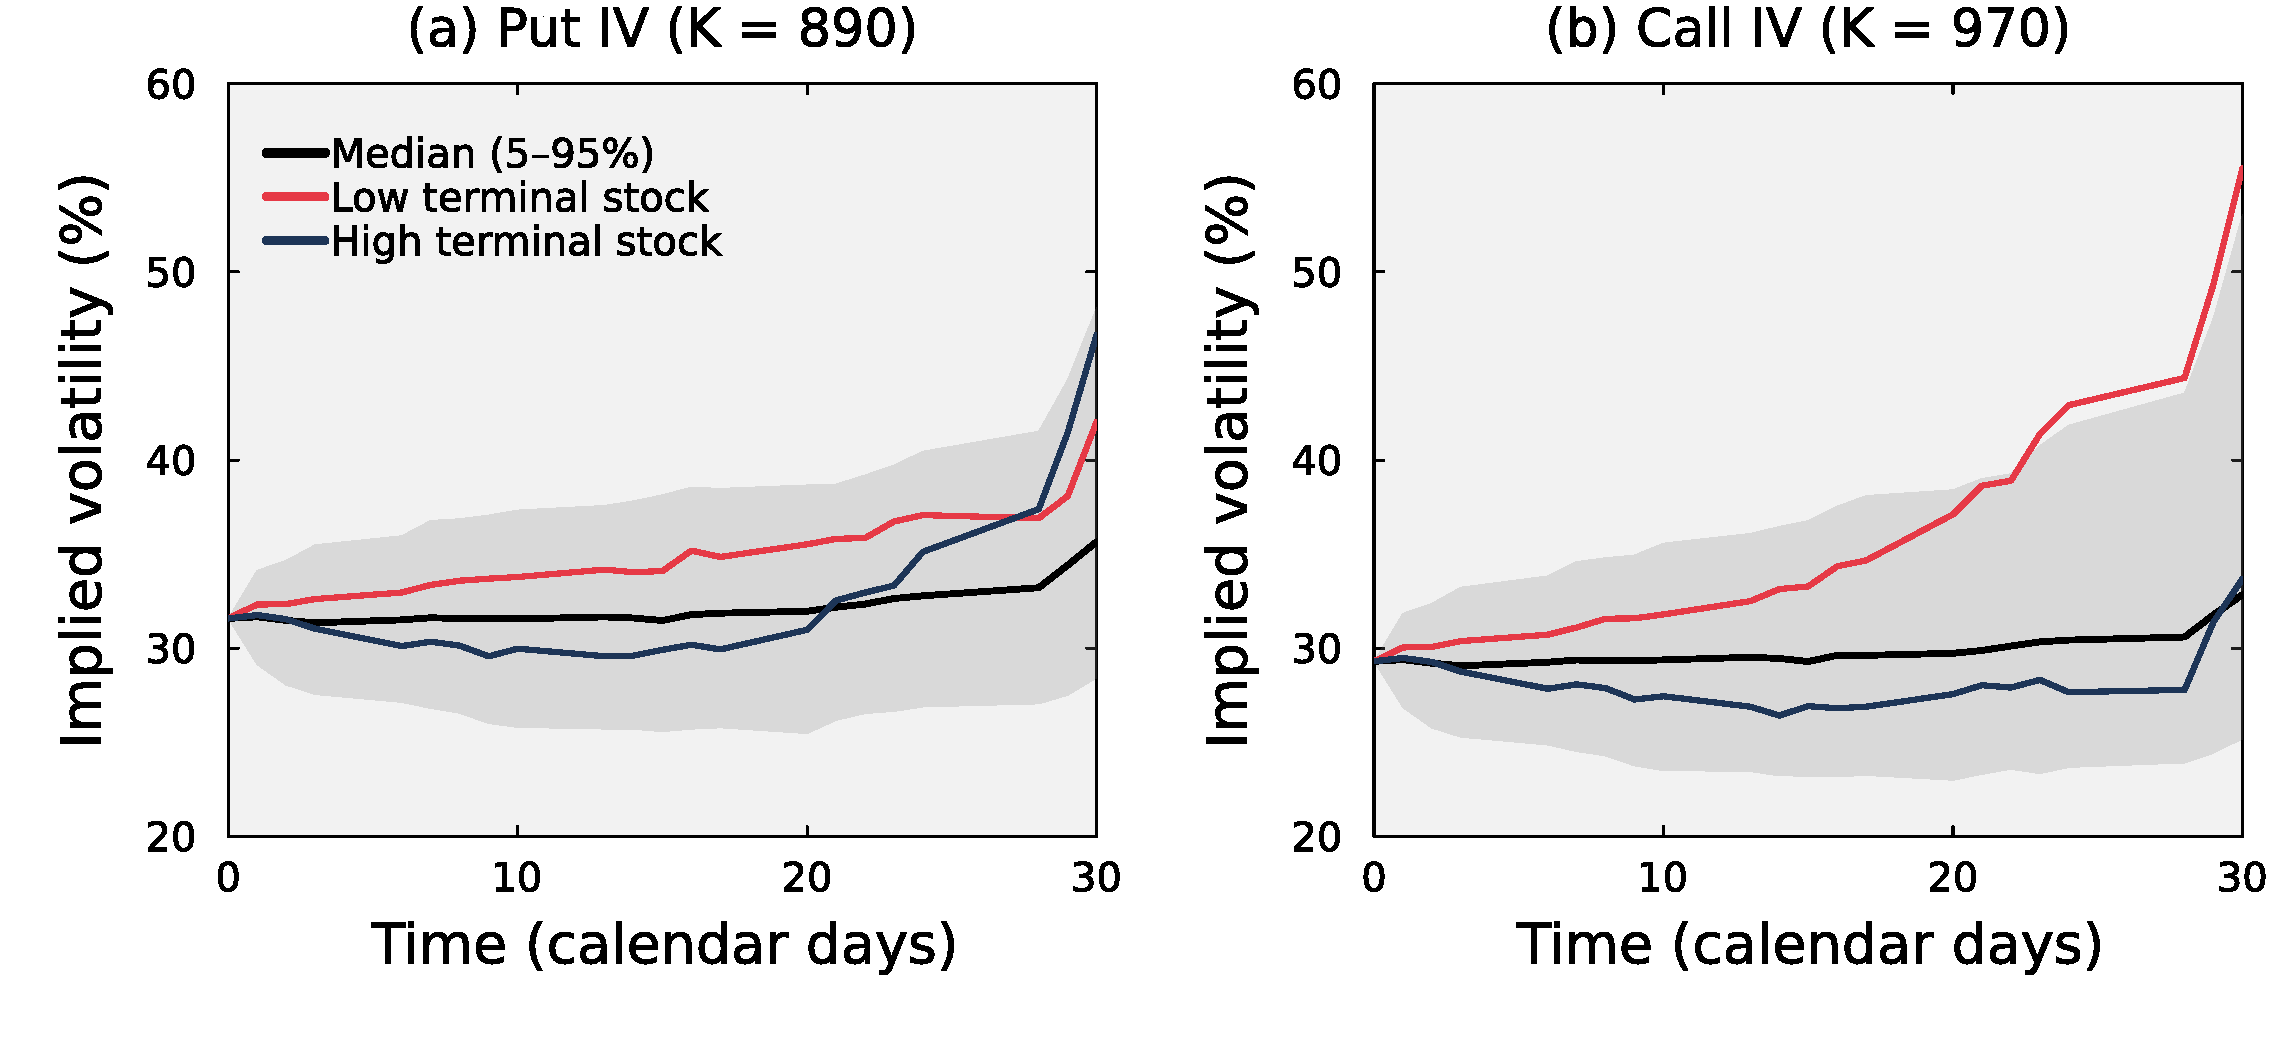
\includegraphics[width=\textwidth]{sections/figures/gs/gs_iv_trajectories.pdf}
\caption{Simulated evolution of annualized IV at the GS put strike (a) and call strike (b). These factors belong to the illustrative scenario in Fig.~\ref{fig:gs_paths}. Both panels express IV as percentages on the same vertical scale. Curves show pointwise medians across all 1{,}000 paths and within the terminal-stock groups defined in Fig.~\ref{fig:gs_paths}; shading shows the 5th--95th percentile band. Time is measured in calendar days from April 28, 2026, and stops before expiration. IV does not enter the expiration payoff.}
\label{fig:gs_iv}
\end{figure}

\FloatBarrier
To measure the contribution of IV dynamics, we compared five variants on identical stock paths for the four scenario contracts. The comparison held contracts, entry premiums, and pricing assumptions fixed so that differences in interim marks could be attributed to the IV module (Section~\ref{sec:ablation_methods}). After ten trading transitions, the full factor changed marks by a mean absolute \$1.77--\$2.41 per share relative to direct surface evaluation (Supplementary Table~\ref{tab:dynamic_ablation}). These pathwise changes were much larger than the corresponding difference in the GS put's mean P\&L, which was only \$0.05 lower under the full factor with a paired Monte Carlo standard error of \$0.04. Positive and negative differences therefore largely canceled when averaged across paths. Frozen IV and deterministic mean reversion also produced different marks from the direct surface, showing that movement of the target and persistence around it affected valuation even without stochastic shocks. Comparing the coupled and uncoupled factors on the same paths showed how return coupling changed valuation across stock outcomes. For both tickers, short-put P\&L declined most on falling-stock paths, while short-call P\&L improved most on rising-stock paths (Fig.~\ref{fig:dynamic_ablation}). Coupling also changed the lower tails of short-position P\&L. We measured those tails with 5\% expected shortfall, defined as mean P\&L at or below its 5\% quantile, for which more negative values indicate larger simulated losses. Negative coupling moved the GS put's expected shortfall from $-\$63.24$ under uncoupled factors to $-\$64.86$ under the full factor. The call's expected shortfall improved from $-\$71.54$ to $-\$69.83$, and the LLY contracts showed the same direction of change (Supplementary Table~\ref{tab:dynamic_ablation}). The full-factor mean absolute mark differences were similar across the three evaluation seeds (Supplementary Table~\ref{tab:ablation_seeds}). All variants produced identical entry marks and terminal payoffs. The experiment thus located the contribution of IV dynamics in interim valuation and liquidation risk while preserving the stock paths and terminal outcomes.

\begin{figure}[H]
\centering

\includegraphics[width=\textwidth]{sections/figures/dynamic_ablation.pdf}
\caption{Effect of return coupling on interim short-option P\&L as a function of stock return after ten trading transitions for (a) GS and (b) LLY. Each difference is coupled-factor P\&L ($\rho=-0.6$) minus uncoupled-factor P\&L ($\rho=0$) on the same stock path, with the same independent normal innovations. Negative values indicate worse short-position P\&L under coupling. The 3{,}000 paths per ticker are sorted by stock return and divided into ten groups of 300. Symbols show median paired P\&L differences at median stock returns; connecting lines guide the eye, and shaded bands span the within-group 25th--75th percentiles. These bands describe variation across paths, not confidence intervals. Red circles denote puts and navy diamonds denote calls. All marks are evaluated on May 12, 2026, with 17 calendar days to expiry.}\label{fig:dynamic_ablation}
\end{figure}

We examined numerical accuracy and strike consistency to determine how the ablation differences should be interpreted as option prices. Increasing lattice depth from 201 to 401 changed sampled marks by at most \$0.0017 per share, well below the differences among IV variants. No factor reached the variance floor in the four scenario contracts. Current strike/spot nevertheless left the training interval on 0.7--2.9\% of pre-expiry path dates across ticker, contract, and seed combinations, so some marks used extrapolated surface values. The strike audit then tested necessary conditions across separately priced contracts. At 401 lattice steps, the direct GS surface exceeded the \$0.01 convexity tolerance in 178 of 1{,}818 tested strike triples (Supplementary Table~\ref{tab:strike_audit}). Its largest excess was \$0.113 per share. The full factor had three monotonicity violations among 2{,}020 adjacent-strike comparisons, with a maximum of \$0.013. These violations persisted at the higher lattice depth, while no LLY variant violated the tested conditions at the stated tolerance. The checks therefore distinguished two issues in the calculation. The sampled ablation effects exceeded the changes from numerical refinement, but single-contract lattice accuracy did not ensure consistency across strikes. The residual GS violations limited the interpretation of the generated prices as market-consistent training data even though the same outputs supported controlled comparisons of IV assumptions.
\FloatBarrier


We used the terminal results to describe the consequences of the selected stock-return models, strikes, and entry premiums (Supplementary Tables~\ref{tab:gs_scenario} and~\ref{tab:lly_scenario}). For a position held to expiration, terminal P\&L was the entry premium minus the payoff determined by the final stock price and strike. In GS, the short put retained its full premium on 74.0\% of paths and the short call did so on 67.6\%. Frequent premium retention nevertheless coexisted with substantial losses: the worst 5\% of put outcomes lost at least \$58.92 per share, and the corresponding call threshold was \$86.24. Those less frequent losses left mean P\&L positive for the put but negative for the call. The market-delta heuristic $1-|\Delta|$ gave premium-retention estimates of 70.5\% and 67.2\% for the same contracts. The LLY put and call retained their premiums on 80.7\% and 79.3\% of paths, respectively, and both had positive mean P\&L under the scenario assumptions. These retention frequencies exceeded the heuristic by 11.0 and 10.2 percentage points. The larger gaps than in GS showed that agreement between the heuristic and simulated strike crossing depended on the ticker and scenario. Quote delta supplied a diagnostic reference from a risk-neutral pricing calculation, whereas the simulated frequencies came from physical stock paths. The terminal results therefore characterized the chosen return distributions and contract inputs. Their independence from interim IV meant that they did not test the fitted surface or the dynamic factor. Evidence for the contribution of IV dynamics came from the paired interim comparisons, which changed the IV module while preserving the stock paths and terminal payoffs.

\FloatBarrier


To examine whether the calibration and simulation results transferred to later observations, we extended the evaluation beyond the original April--May window. The completed expanding-window experiment evaluated two-input sector networks on 53 successive held-out capture dates through July 17. Median test RMSE was 9.92 IV percentage points, but individual folds ranged from 7.68 to 19.25 points (Supplementary Table~\ref{tab:walk_forward_extended}). This spread showed that the pooled surface representation transferred unevenly across dates. Each fold used the later observation's stock price to determine moneyness, so the result concerned conditional IV prediction rather than a forecast of the stock--option system. We then fitted a single set of sector surfaces through July 31 and evaluated the 23 later sessions from August 4 through September 4. Pooled RMSE increased from 10.79 points in training to 14.75 points in the held-out sample (Supplementary Table~\ref{tab:chronological_surface}). These values were not a paired comparison with the earlier folds because the fitting window, capture audit, and evaluation dates differed. The GS surface had held-out RMSE of 6.30 points and mean overprediction of 0.88 points, whereas LLY had RMSE of 9.96 points and mean overprediction of 4.61 points. The larger corpus therefore did not remove the problem of a frozen surface level lagging a later market state. This motivated a separate forecast comparison in which all IV variants started from the observed origin IV and differed in their subsequent evolution (Section~\ref{sec:chronological_methods}).

The forward evaluation compared forecasts with later observations of the same selected contracts. The maturity-bucket collection scheme imposed an immediate limit: none of the 36 eligible roughly monthly contracts per ticker had an observed exact-symbol endpoint after five sessions (Supplementary Table~\ref{tab:forecast_availability}). Their one-session comparison retained 34 quotes across 17 origins per ticker. Coupled-factor MAE was \$3.79 per share for GS and \$6.08 for LLY, compared with \$3.80 and \$6.11 under frozen IV (Supplementary Table~\ref{tab:forecast_one_session}). The separately identified shorter-maturity cohort supplied five-session outcomes for 34 GS and 30 LLY quotes across 17 origins per ticker. Coupling again produced only small reductions in absolute error of the forecast mean: MAE was \$4.19 versus \$4.21 under frozen IV for GS, and \$11.59 versus \$11.62 for LLY (Table~\ref{tab:forecast_main}). It improved the date-level mean absolute error on six of seventeen GS origins and nine of seventeen LLY origins, so the small average reductions did not show a consistent advantage across dates. Scoring forecast medians separately lowered GS coupled-factor MAE to \$2.48 and gave LLY MAE of \$11.79, with little separation from frozen IV (Supplementary Table~\ref{tab:option_point_summary}). The coupled model's CRPS was 2.01 for GS and 8.93 for LLY, compared with 2.02 and 8.99 under frozen IV. Central 90\% intervals had date-weighted coverage of 100\% for GS and 67.6\% for LLY, with average widths of \$25.65 and \$28.91 per share. Broad coverage in GS therefore coexisted with substantial missed coverage in LLY. The earliest eligible GS example showed nearly coincident coupled and frozen-IV mean forecasts while the observed call value declined below both means (Fig.~\ref{fig:chronological_forecast}). These results supported a limited chronological case study of the assembled model, but they did not establish a material forecasting advantage from the fixed stochastic factor or validate the original month-long illustrations.

\begin{table}[H]
\centering
\caption{Five-session option forecasts for the shorter-maturity cohort, selected with 10--21 calendar DTE at each origin. Scores average matched contracts within each ticker and origin before averaging dates. MAE scores the forecast mean; MAE, CRPS, and central 90\% interval width are dollars per share. Coverage is date-weighted. Every IV variant uses the same stock paths, origin IV, and matched quotes.}\label{tab:forecast_main}
\resizebox{\textwidth}{!}{\begin{tabular}{llrrrrrr}
\toprule
Ticker & IV variant & Dates & Quotes & MAE & CRPS & Coverage (\%) & Width \\
\midrule
GS & Frozen IV & 17 & 34 & 4.21 & 2.02 & 100.0 & 25.64 \\
GS & Direct surface & 17 & 34 & 4.86 & 2.16 & 67.6 & 24.01 \\
GS & Mean reversion & 17 & 34 & 4.26 & 2.02 & 100.0 & 25.62 \\
GS & Uncoupled factor & 17 & 34 & 4.24 & 2.03 & 100.0 & 25.69 \\
GS & Coupled factor & 17 & 34 & 4.19 & 2.01 & 100.0 & 25.65 \\
LLY & Frozen IV & 17 & 30 & 11.62 & 8.99 & 73.5 & 28.98 \\
LLY & Direct surface & 17 & 30 & 11.62 & 9.05 & 55.9 & 26.68 \\
LLY & Mean reversion & 17 & 30 & 11.62 & 8.99 & 73.5 & 28.83 \\
LLY & Uncoupled factor & 17 & 30 & 11.61 & 8.97 & 73.5 & 28.83 \\
LLY & Coupled factor & 17 & 30 & 11.59 & 8.93 & 67.6 & 28.91 \\
\bottomrule\end{tabular}
}
\end{table}

\begin{figure}[H]
\centering
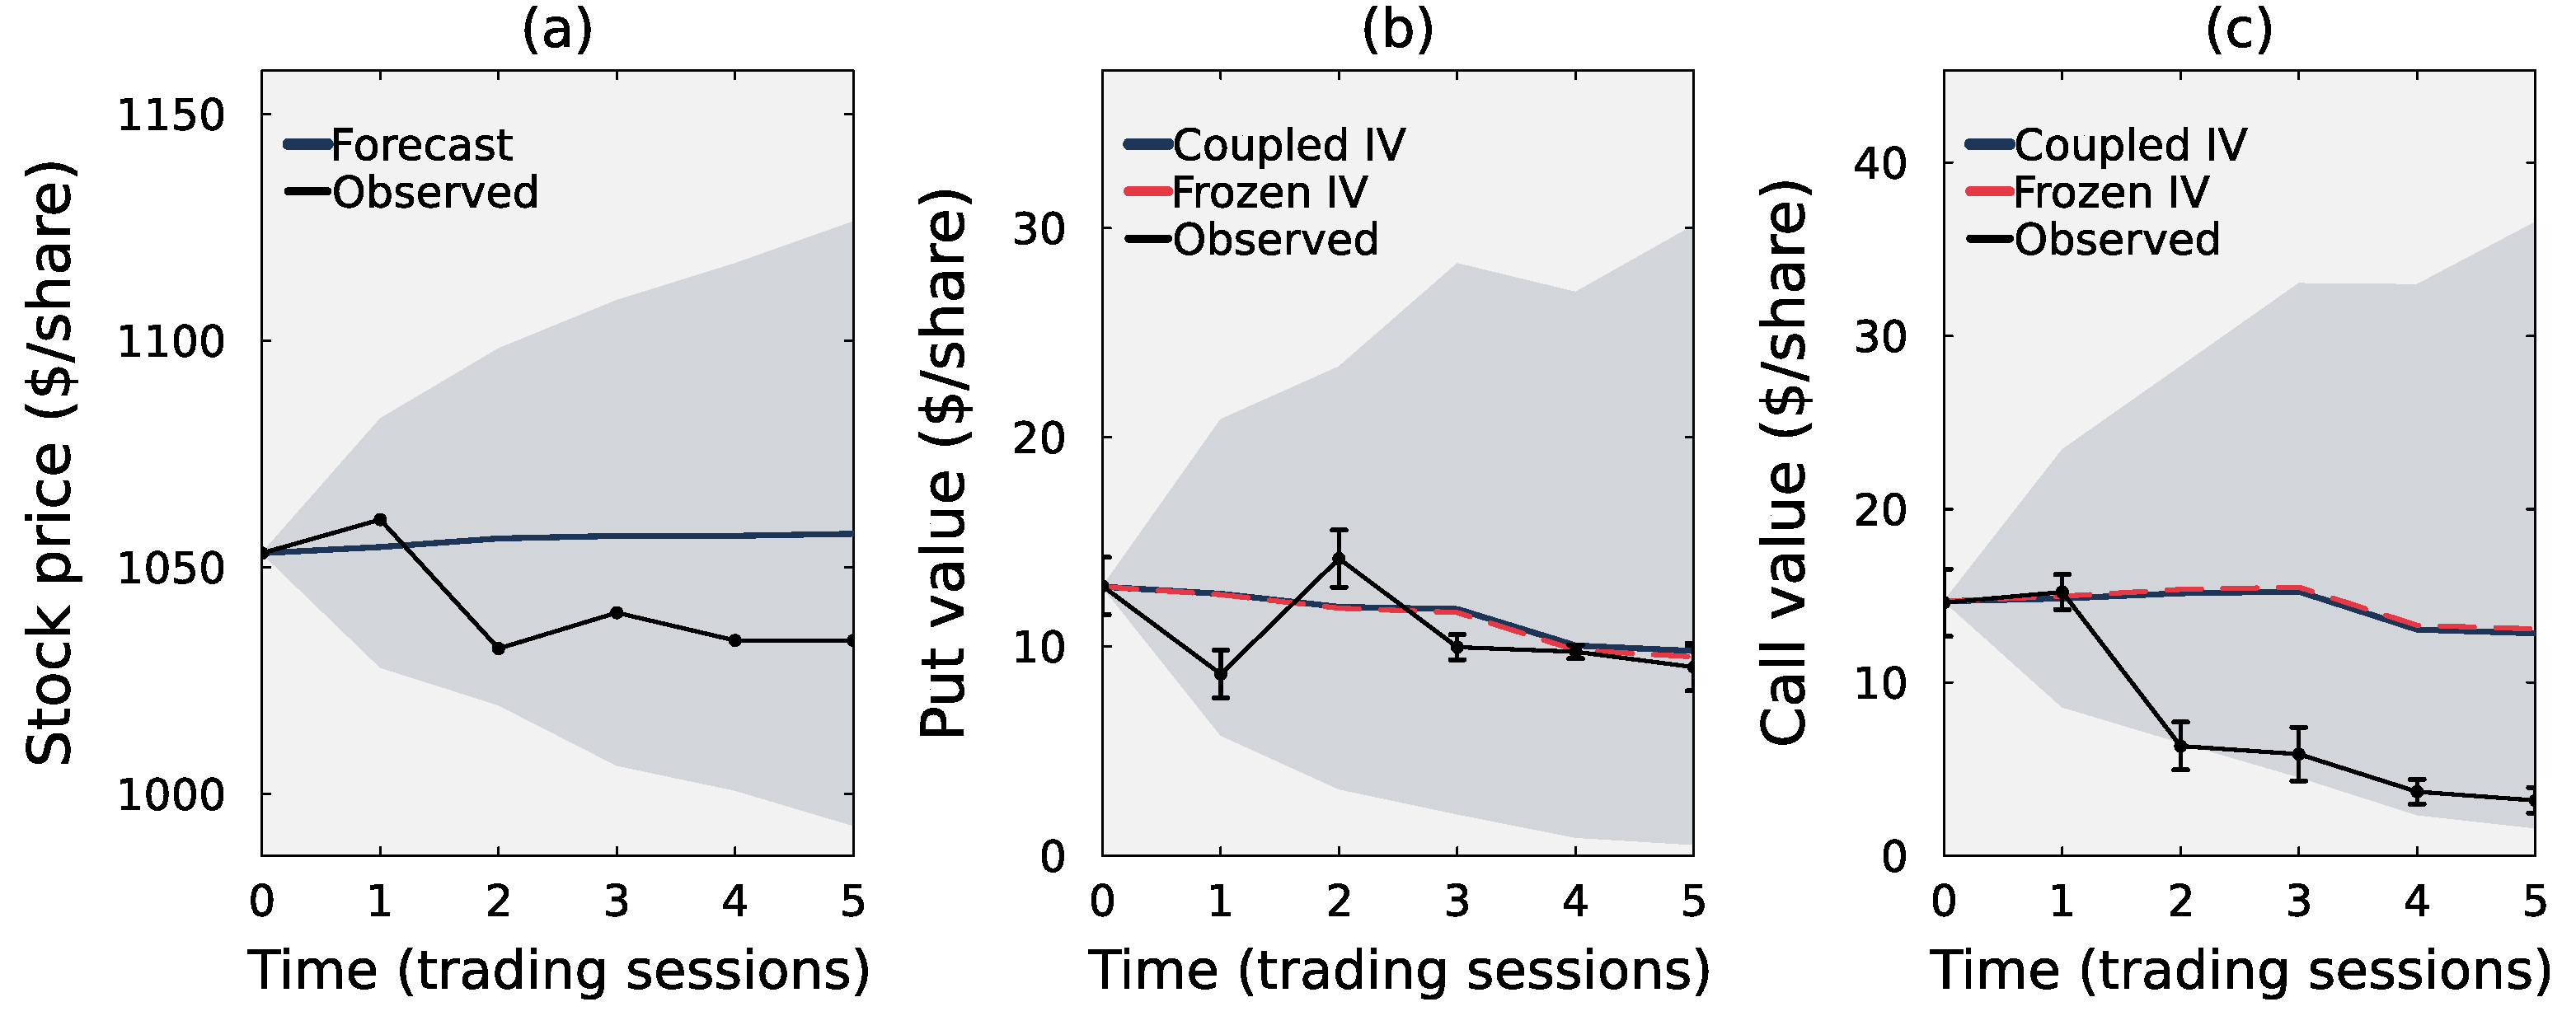
\includegraphics[width=\textwidth]{sections/figures/chronological_forecast.pdf}
\caption{Five-session forecasts of GS stock prices (a), put values (b), and call values (c), compared with observations from August 4 to August 11, 2026. The put strike is \$1{,}000, the call strike is \$1{,}105, and both contracts expire on August 21. Forecasts use the July-cutoff surface and information available at the August 4 origin. Navy curves show forecast means from 1{,}000 stock paths, with the coupled IV factor used for option values; shading spans the central 90\% of simulated values. Red dashed curves show frozen-IV mean option forecasts on the same stock paths. Black points show observed stock closes and option midpoints, with vertical bars spanning Alpaca's indicative bid and ask. These option observations are vendor values rather than exchange quotes. Time is measured in exchange sessions from the origin. This is the earliest GS origin with both selected shorter-maturity contracts observed at the five-session endpoint.}\label{fig:chronological_forecast}
\end{figure}

We used the observed-stock diagnostic to distinguish stock-path errors from the IV and pricing components on a common subset. Complete intervening stock observations were available for thirteen five-session origins per ticker, with 26 matched GS quotes and 24 LLY quotes. On these same cases, replacing simulated stock paths with the observed path reduced coupled-factor MAE from \$4.62 to \$1.23 per share for GS and from \$10.61 to \$1.95 for LLY. The observed path was supplied after the forecast period and would have been unknown at the origin. This calculation diagnosed error sources; it was not an attainable improvement to the forward forecast. Within that diagnostic, frozen IV had lower point errors of \$1.07 and \$1.74, while uncoupled stochastic factors had lower CRPS than the coupled factor for both tickers (Supplementary Table~\ref{tab:forecast_conditional}). The stock comparison also gave no point-forecast advantage to the retained JumpHMM settings: five-session stock MAE was \$16.85 for GS and \$49.83 for LLY, versus \$16.17 and \$48.64 for the simple random walk (Supplementary Table~\ref{tab:forecast_stock}). Repricing the shorter-maturity endpoint observations with their reported IV reduced five-session option MAE to \$0.14 for GS and \$0.34 for LLY, and those prices lay within every observed bid--ask interval (Supplementary Table~\ref{tab:forecast_repricing}). Sampled lattice refinement changed marks by at most \$0.0026 per share across the two cohorts, well below the forecast errors. Together, these diagnostics showed that stock-forecast errors contributed substantially to the option-price misses, with additional error remaining in the IV and pricing inputs. They did not establish why the stock estimator missed or how to correct it. They did not identify a reliably superior dynamic variant. The small, overlapping set of origins, missing contract histories, fixed parameters, and absence of quote-level exchange timestamps limited broader conclusions about forecasting accuracy or executable trading performance.
The wider return-cutoff comparison repeated the same chronological forecasts and stock benchmarks. Widening the residual bound from $b=10$ to $b=20$ changed five-session coupled option MAE by less than \$0.007 per share and the reported stock CRPS values by less than \$0.002 (Supplementary Table~\ref{tab:tail_forecasts}). These changes did not alter the conclusions of the specified forecast comparisons.
\FloatBarrier

The reduction in option errors after supplying the observed stock path raised a separate question: could a change to the stock forecast improve predictions without using future information? Return-scaling checks and reconstruction of the saved paths found no error in the conversion from annualized log growth to daily prices. Conditioning the initial state on recent returns also did not materially improve five-session central forecasts. Median-based stock MAE changed from \$16.28 to \$16.36 for GS and from \$49.58 to \$49.40 for LLY in that diagnostic (Supplementary Table~\ref{tab:stock_initialization}). The effect of the initial state on the forecast distribution largely disappeared within a few sessions under the fitted transitions. We then compared the retained JumpHMM with unchanged-price, adaptive-volatility, and simple directional benchmarks, using earlier data to select the new models' settings. Validation across 2019--2024 selected an EWMA decay of $0.97$ and the zero-drift limit of the directional regression (Supplementary Table~\ref{tab:stock_selection}). The selected directional and adaptive forecasts were consequently identical. The stock and SPY return features did not justify a directional adjustment under this selection criterion. Testing the frozen models in 2025 supplied 245 five-session origins per ticker, substantially more than the 17 available in the 2026 case study. Across these comparisons, central price errors remained close to the unchanged-price benchmark (Table~\ref{tab:stock_validation}). These results did not establish a repair for the large stock-price misses or a consistent central-forecast advantage from the added predictors.

\begin{table}[H]
\centering
\caption{Five-session stock forecasts in 2025 and August--September 2026. Each ticker has 245 origins in 2025 and 17 in 2026. MAE scores the forecast median; MAE, CRPS, and central 90\% interval width are dollars per share. Scores average dates within each of three 10{,}000-path replicates and then average replicates. Adaptive denotes the Gaussian model with historically selected EWMA decay $0.97$. Historical selection chose zero directional drift, making the selected directional model identical to Adaptive. The unchanged-price benchmark has no uncertainty interval.}\label{tab:stock_validation}
\resizebox{\textwidth}{!}{\begin{tabular}{lllrrrr}
\toprule
Year & Stock & Model & Median MAE & CRPS & Coverage (\%) & Width \\
\midrule
2025 & GS & JumpHMM & 22.31 & 16.22 & 84.4 & 84.71 \\
2025 & GS & Unchanged & 22.61 & 22.61 & -- & -- \\
2025 & GS & Adaptive & 22.62 & 16.32 & 89.8 & 94.86 \\
2025 & LLY & JumpHMM & 39.10 & 29.60 & 69.9 & 100.40 \\
2025 & LLY & Unchanged & 39.37 & 39.37 & -- & -- \\
2025 & LLY & Adaptive & 39.35 & 28.57 & 84.4 & 151.37 \\
2026 & GS & JumpHMM & 16.25 & 13.03 & 100.0 & 129.05 \\
2026 & GS & Unchanged & 15.51 & 15.51 & -- & -- \\
2026 & GS & Adaptive & 15.48 & 15.58 & 100.0 & 176.18 \\
2026 & LLY & JumpHMM & 49.44 & 35.60 & 70.6 & 147.26 \\
2026 & LLY & Unchanged & 49.37 & 49.37 & -- & -- \\
2026 & LLY & Adaptive & 49.31 & 33.81 & 94.1 & 191.38 \\
\bottomrule
\end{tabular}
}
\end{table}

The stock-distribution comparison nevertheless identified a narrower benefit from adaptive volatility. In 2025, LLY's five-session CRPS fell from 29.60 under JumpHMM to 28.57 under the adaptive model, while central 90\% coverage increased from 69.9\% to 84.4\%. Average interval width increased from \$100.40 to \$151.37, so the coverage gain came with a wider range of predicted prices. The lower CRPS indicated that this tradeoff improved the distribution score, although coverage remained below its nominal level. The 2026 comparison showed the same direction of change for LLY: CRPS fell from 35.60 to 33.81 and coverage rose from 70.6\% to 94.1\% (Table~\ref{tab:stock_validation}). The adaptive model had lower date-level CRPS on 131 of 245 LLY origins in 2025 and ten of seventeen in 2026. For GS, however, CRPS increased slightly in 2025, from 16.22 to 16.32, and more substantially in 2026, from 13.03 to 15.58. Both GS models covered every 2026 endpoint, but the adaptive intervals were wider. Full five-session results, including mean-based RMSE and the identical selected directional forecasts, are given in Supplementary Table~\ref{tab:stock_validation_five}. The one-session comparison also showed little separation in central price error from an unchanged-price forecast (Supplementary Table~\ref{tab:stock_validation_one}). The findings therefore supported a ticker-dependent improvement in forecast uncertainty for LLY, not a general improvement in predicting stock-price direction. We retained JumpHMM as the worked example for the IV framework and did not select a replacement stock model from these test outcomes.
\FloatBarrier

